\documentclass[border=5pt]{standalone}
\usepackage{tikz,graphicx,amsmath,amssymb,xcolor}\usepackage{fontspec,xeCJK}\setmainfont{Helvetica}\setCJKmainfont{PingFang SC}
\usetikzlibrary{arrows.meta}
\definecolor{ink}{HTML}{203D46}\definecolor{teal}{HTML}{277A80}\definecolor{pale}{HTML}{EFF6F5}\definecolor{warm}{HTML}{F6ECDD}\definecolor{training}{HTML}{BB7347}
\begin{document}\begin{tikzpicture}[x=1mm,y=1mm,font=\fontsize{11}{14}\selectfont,text=ink]
\path[use as bounding box] (-11,0) rectangle (120,260);
\node[anchor=north west,font=\bfseries\fontsize{16}{19}\selectfont] at (3,258) {SAM 2：一张图走完整条链};
\node[anchor=north west,text width=98mm,font=\fontsize{10}{13}\selectfont] at (3,248) {运行：$A\to B\to C\to D$，记忆回 B。E 单独监督；本文采用 arXiv v2 的 SAM 2.1 权重结果。};
\fill[pale,rounded corners=2mm] (1,191) rectangle (104,232);
\node[anchor=north west,text=teal,font=\bfseries\fontsize{12}{15}\selectfont] at (4,230) {A 当前帧 · §4};
\node[anchor=north west,text width=66mm,inner sep=0] at (4,222) {$1024^2$ 图像 $\rightarrow$ Hiera + FPN\\主特征 $256\times64\times64$\\高分辨率特征旁路到解码器\\一帧编码，多目标共享};
\node[anchor=center,inner sep=0] at (88,208) {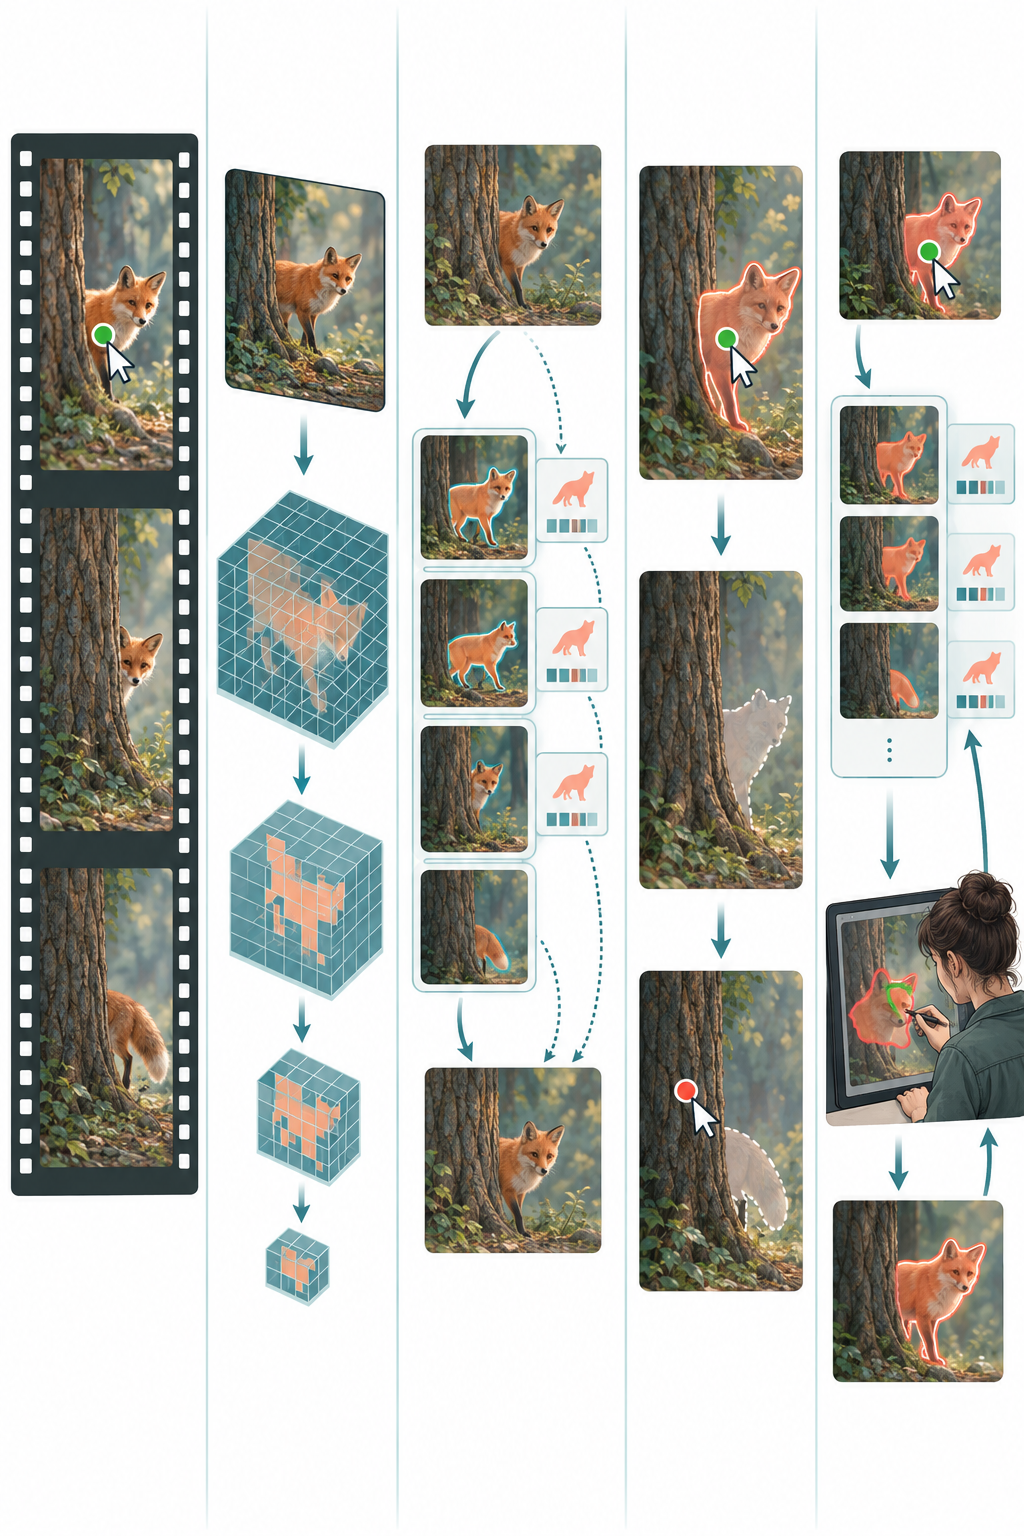
\includegraphics[width=26mm,height=31mm,keepaspectratio,viewport=209 206 390 1416,clip]{sam2-imagegen-draft.png}};
\draw[-{Latex[length=2mm]},teal,line width=.7pt] (52.5,190.5) -- (52.5,187);
\fill[pale,rounded corners=2mm] (1,145) rectangle (104,186);
\node[anchor=north west,text=teal,font=\bfseries\fontsize{12}{15}\selectfont] at (4,184) {B 翻对象记忆 · §4 / 附录 D};
\node[anchor=north west,text width=66mm,inner sep=0] at (4,176) {4 层：自注意力 $\to$ 跨注意力\\读取空间记忆、对象指针\\近期 6 帧 + 提示帧记忆\\当前图像结合对象历史};
\node[anchor=center,inner sep=0] at (88,162) {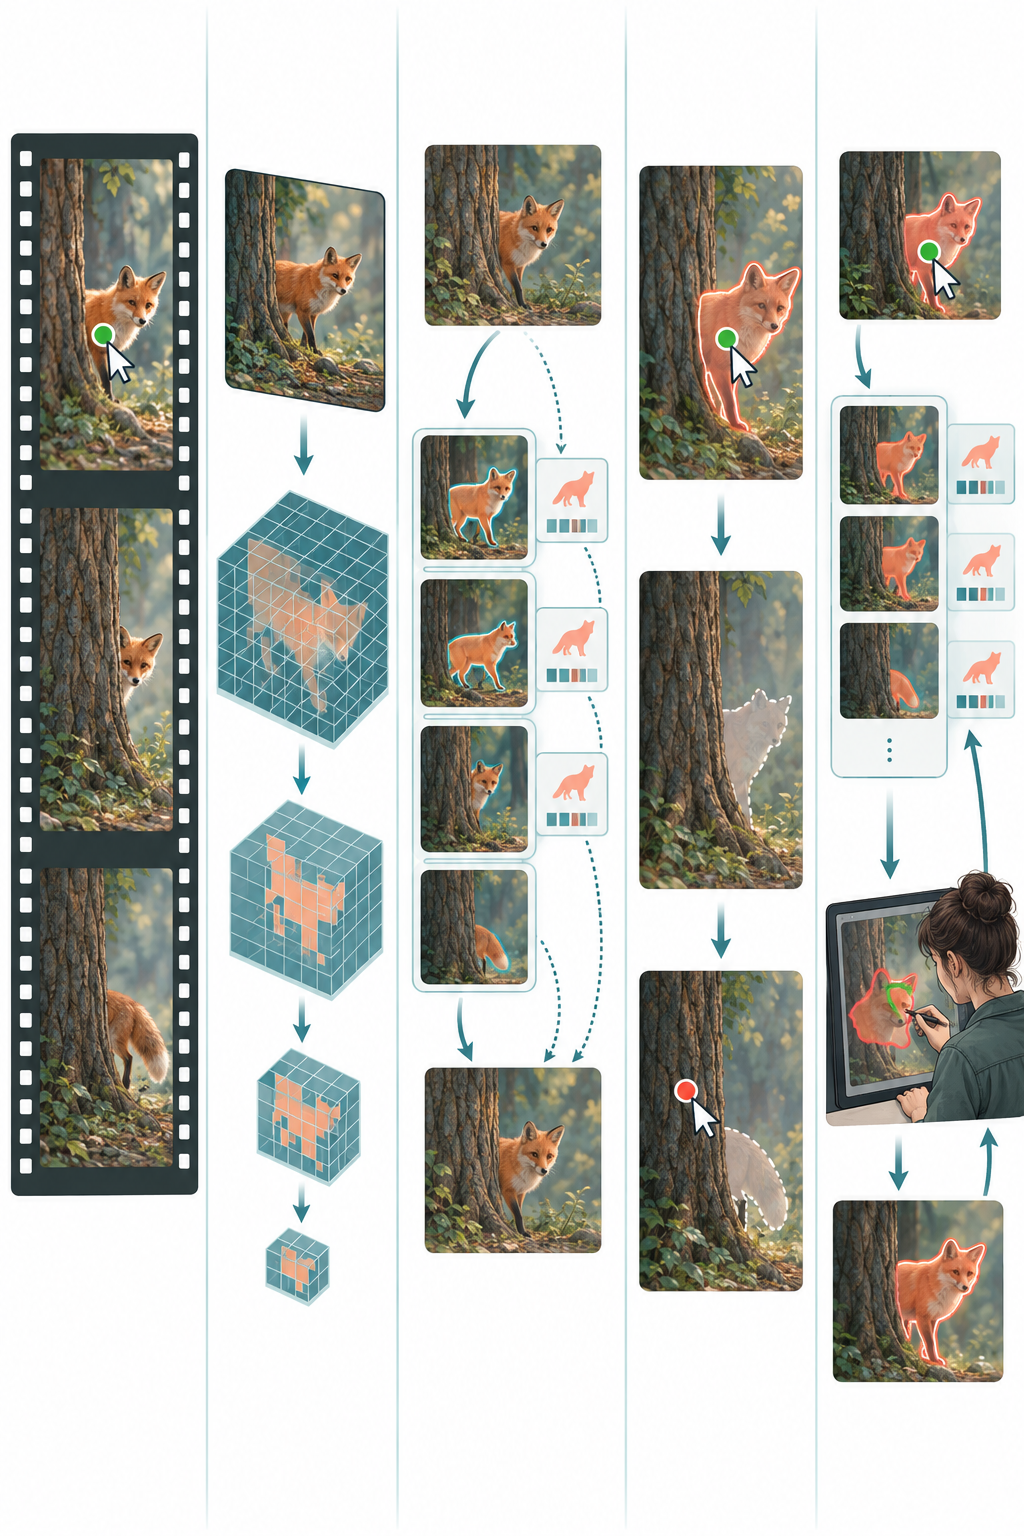
\includegraphics[width=26mm,height=31mm,keepaspectratio,viewport=410 276 608 1396,clip]{sam2-imagegen-draft.png}};
\draw[-{Latex[length=2mm]},teal,line width=.7pt] (52.5,144.5) -- (52.5,141);
\fill[pale,rounded corners=2mm] (1,99) rectangle (104,140);
\node[anchor=north west,text=teal,font=\bfseries\fontsize{12}{15}\selectfont] at (4,138) {C 提示到掩码 · §3–4};
\node[anchor=north west,text width=66mm,inner sep=0] at (4,130) {点击 / 框 / 掩码编码\\双向解码器预测多个掩码\\IoU 评分选择候选\\存在性头判断遮挡 / 缺席};
\node[anchor=center,inner sep=0] at (88,116) {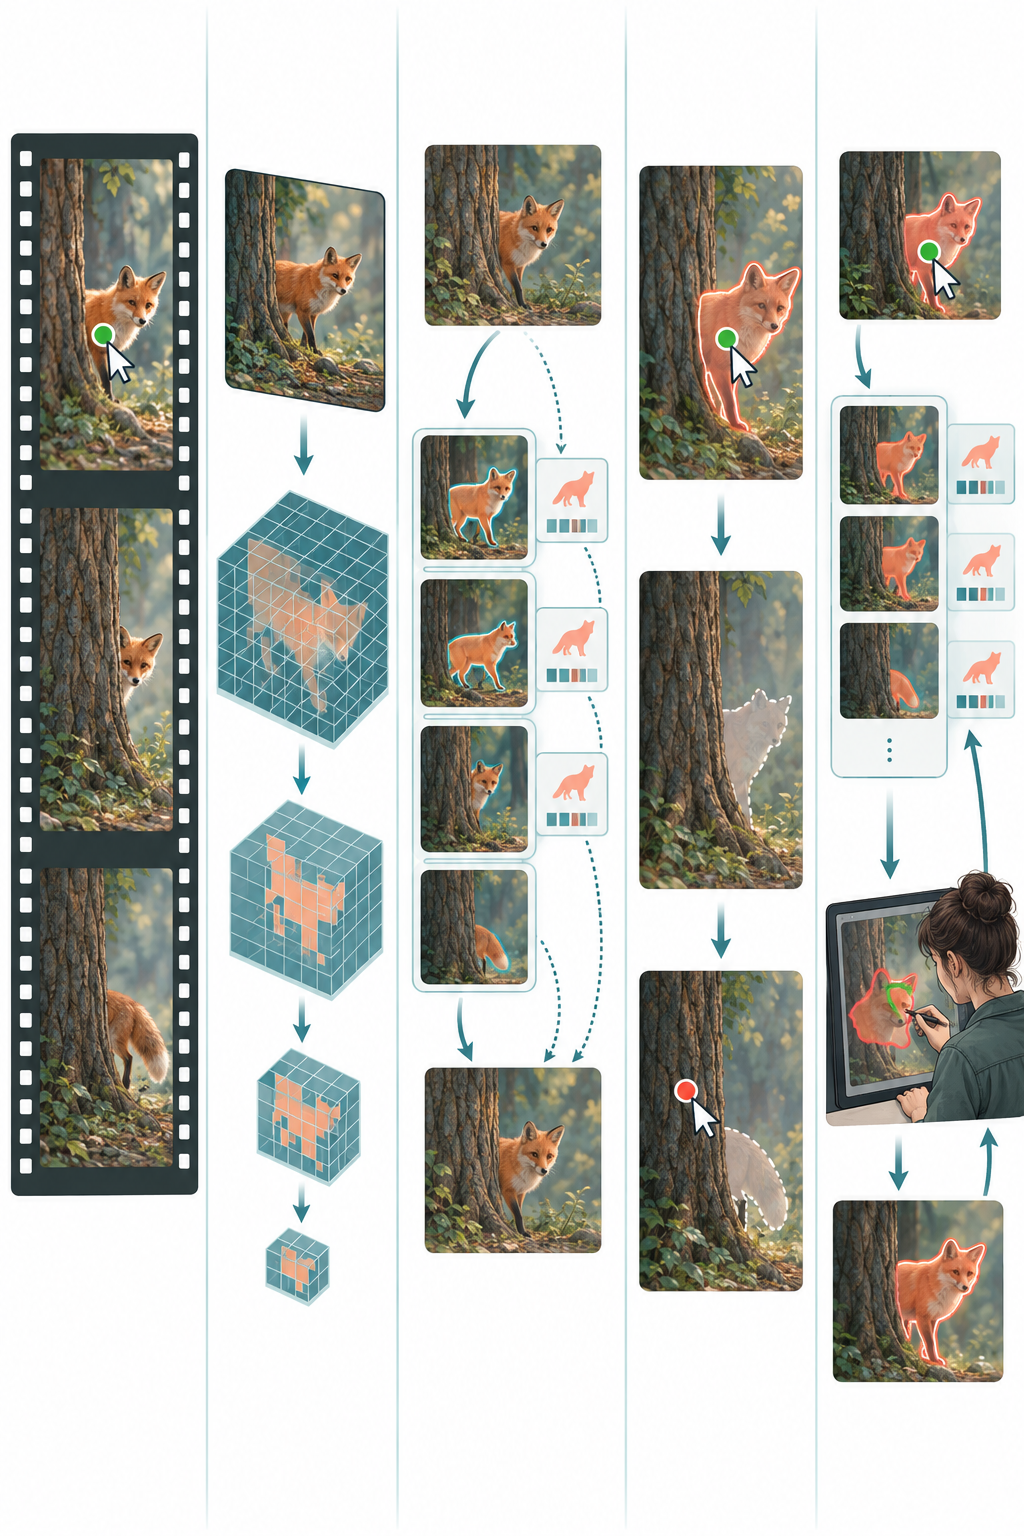
\includegraphics[width=26mm,height=31mm,keepaspectratio,viewport=625 240 820 1385,clip]{sam2-imagegen-draft.png}};
\draw[-{Latex[length=2mm]},teal,line width=.7pt] (52.5,98.5) -- (52.5,95);
\fill[pale,rounded corners=2mm] (1,53) rectangle (104,94);
\node[anchor=north west,text=teal,font=\bfseries\fontsize{12}{15}\selectfont] at (4,92) {D 更新记忆 · §4};
\node[anchor=north west,text width=66mm,inner sep=0] at (4,84) {原始图像特征 + 当前预测掩码\\卷积融合、压到 64 通道\\对象指针：256 维\\新记忆服务下一帧 B 区};
\node[anchor=center,inner sep=0] at (88,70) {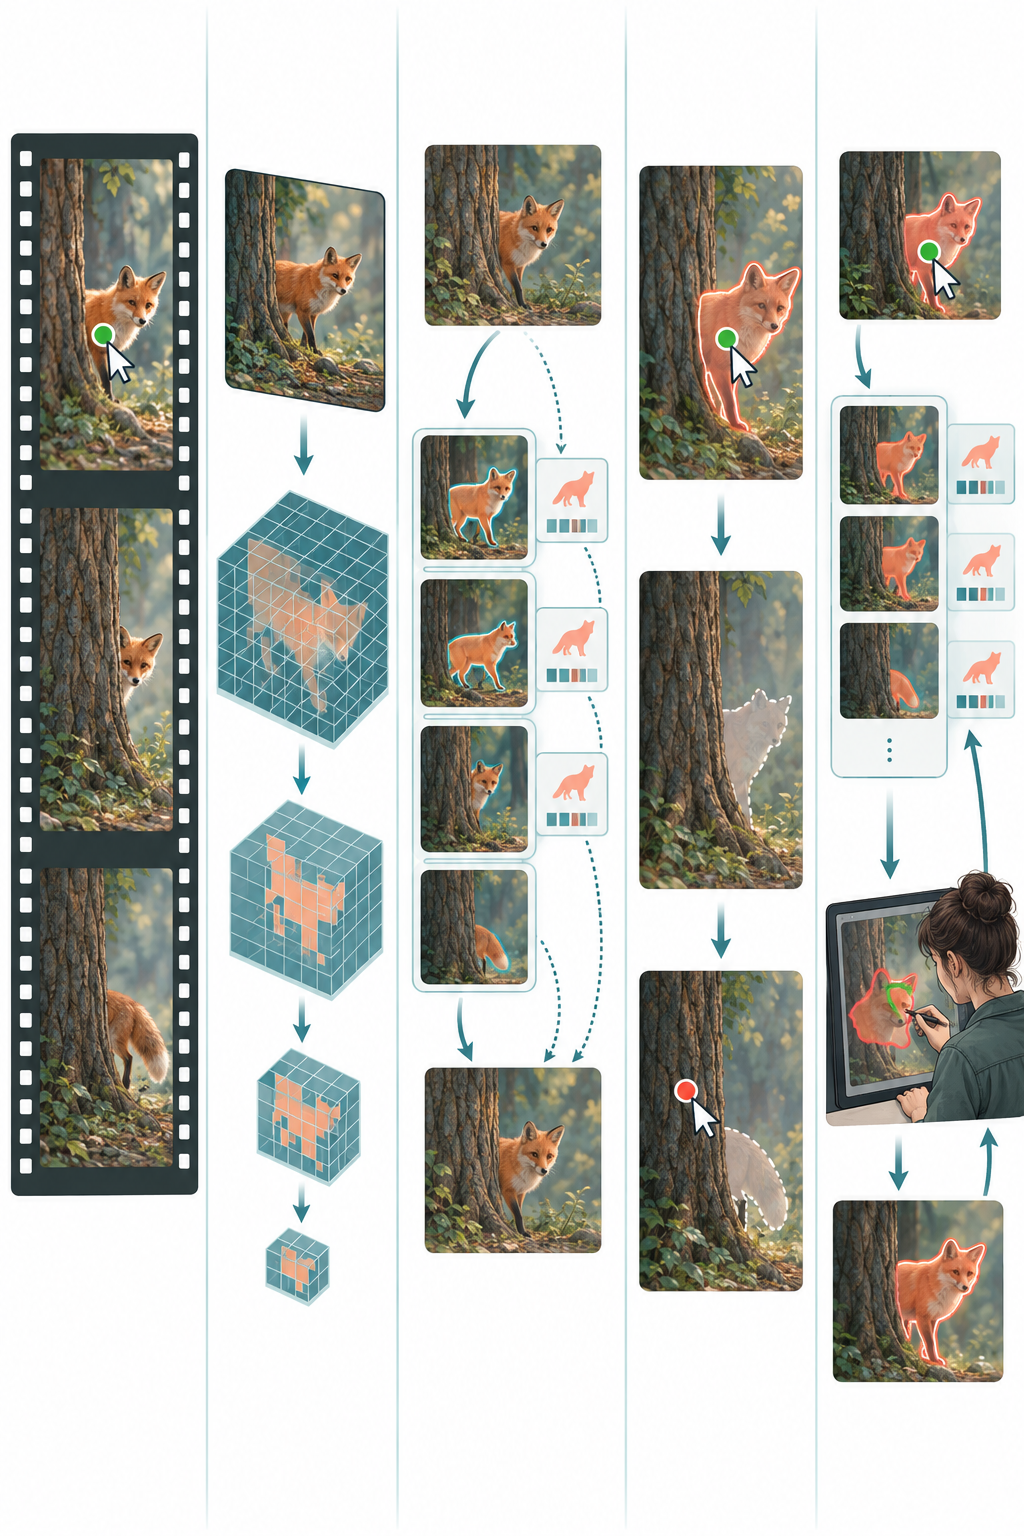
\includegraphics[width=26mm,height=31mm,keepaspectratio,viewport=830 153 1024 1396,clip]{sam2-imagegen-draft.png}};

\fill[warm,rounded corners=2mm] (1,7) rectangle (104,48);
\node[anchor=north west,text=teal,font=\bfseries\fontsize{12}{15}\selectfont] at (4,46) {E 训练与评测 · §5–7};
\node[anchor=north west,text width=66mm,inner sep=0] at (4,38) {人工纠正 $\rightarrow$ 更好训练样本\\掩码 / IoU / 存在性监督\\图像与视频联合训练\\比较精度、交互次数、速度};
\node[anchor=center,inner sep=0] at (88,24) {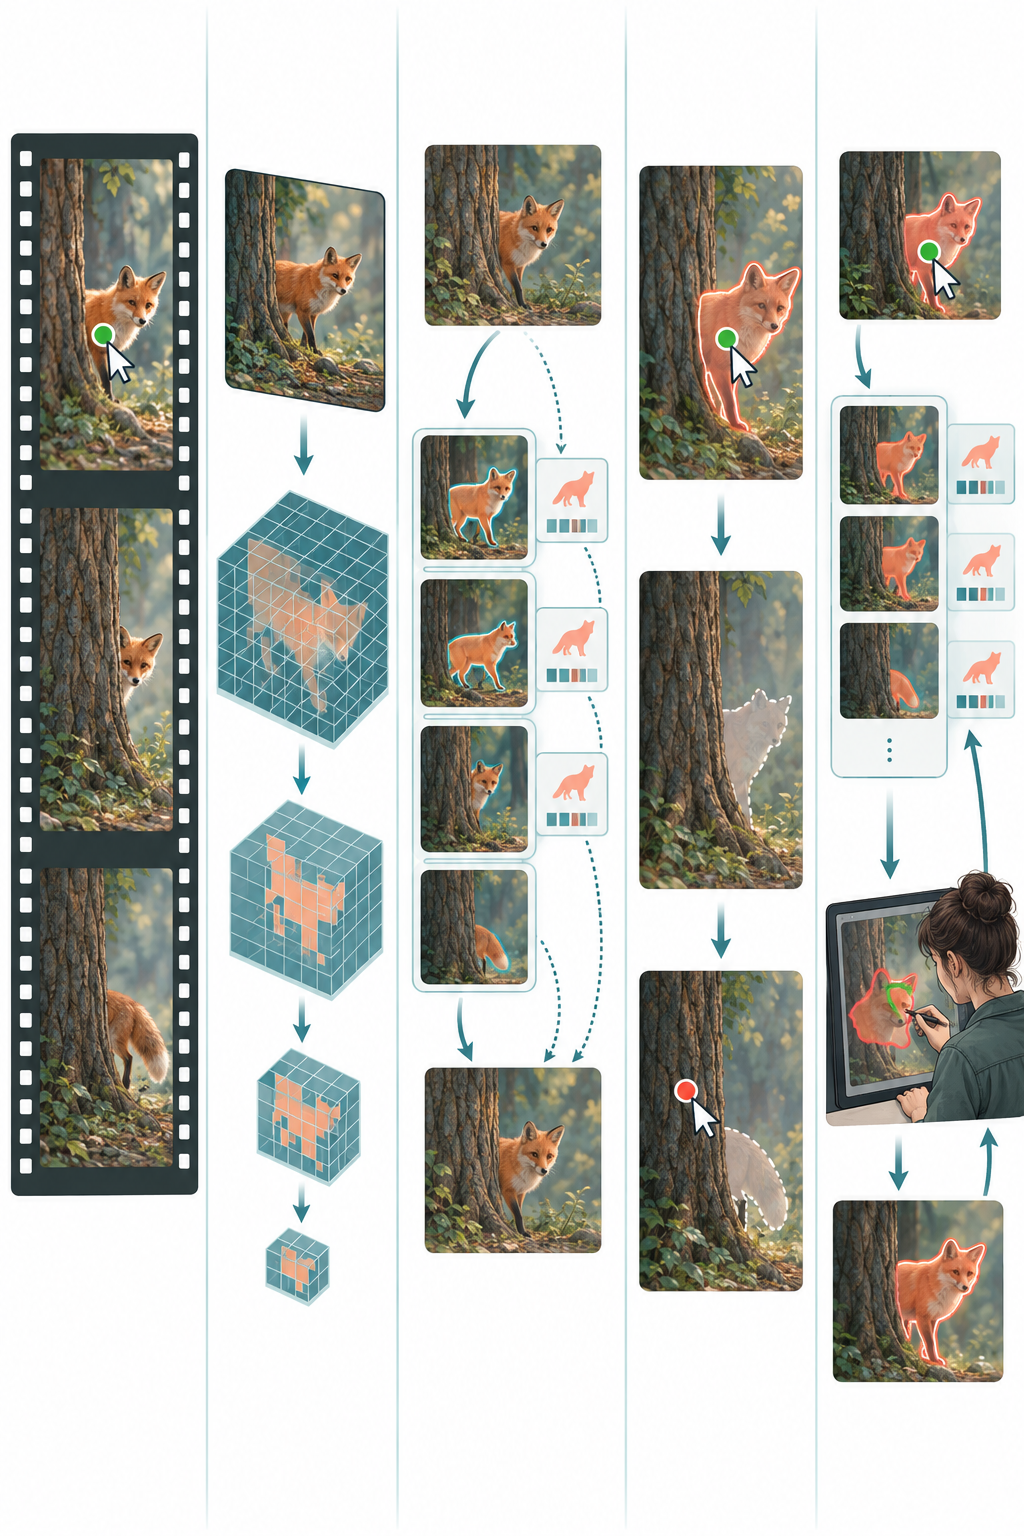
\includegraphics[width=26mm,height=31mm,keepaspectratio,viewport=0 339 201 1416,clip]{sam2-imagegen-draft.png}};
\draw[-{Latex[length=2mm]},teal,line width=.8pt] (104,74) -- (111,74) -- (111,164) -- (104,164);
\node[rotate=90,text=teal,font=\fontsize{9}{11}\selectfont,fill=white,inner sep=1pt] at (114,119) {D 到 B：下一帧对象记忆};
\draw[-{Latex[length=2mm]},training,dashed,line width=.9pt] (1,28) -- (-5,28) -- (-5,119) -- (1,119);
\node[rotate=90,text=training,font=\fontsize{8}{10}\selectfont,fill=white,inner sep=1pt] at (-7,74) {E：独立训练监督，损失回传};
\end{tikzpicture}\end{document}